\documentclass[a4paper,12pt]{article}
\usepackage[utf8]{inputenc}
\usepackage[ngerman]{babel}
\usepackage[T1]{fontenc}
\usepackage[scaled]{uarial}
\usepackage{amsmath}
\usepackage{titling}
\usepackage{fancyhdr}
\usepackage{calc}
\usepackage[a4paper, margin=2.5cm]{geometry}
\usepackage{tocloft}
\usepackage{graphicx}
\usepackage{caption}
\usepackage{acronym}
\usepackage{upquote}
\usepackage[style=authoryear,backend=biber]{biblatex}
\addbibresource{Literature.bib}
\usepackage{csquotes}
\usepackage{filecontents}
\usepackage{setspace}
\usepackage{ragged2e}
\usepackage[backend=biber]{biblatex}
\usepackage{framed}
\usepackage{tabularx}
\usepackage{geometry}
\usepackage{fancyhdr}
\usepackage{enumitem}
\usepackage[parfill]{parskip}

\setlength\bibnamesep{1.5\itemsep}
\renewcommand{\cftsecleader}{\cftdotfill{\cftdotsep}}
\linespread{1.5}
\pagestyle{fancy}
\renewcommand*\familydefault{\sfdefault}
\fancyhf{}
\setlength{\parskip}{6pt}
\onehalfspacing
\justifying
\fancyhead[L]{Einsatz von GenAI-Technologien zur Bewertung von Antworten}
\cfoot{\tiny Studienarbeit / Stand \today \hfill \thepage}
\title{Einsatz von GenAI-Technologien zur Bewertung von Antworten}
\author{Len Vejsada}
\date{\today}
\geometry{a4paper, margin=1in}
\setlength{\parindent}{0pt}


\renewcommand{\maketitle}{
  \begin{center}
    {\LARGE\textbf{\thetitle}}\\[2em]
    {{Studienarbeit\\[2em]
     des Studiengangs Informatik\\[0.5em]
     an der \\[0.5em]
     Dualen Hochschule Baden-Württemberg Karlsruhe\\[0.5em]
     von}}\\[1em]
    \theauthor\\[1em]
    \thedate\\[7em]
  \end{center}
}

\fancypagestyle{firstpage}{
  \fancyhf{}
  \renewcommand{\headrulewidth}{0pt}
  \cfoot{\tiny Studienarbeit / Stand \today \hfill \thepage}
}


\begin{document}
\thispagestyle{firstpage}
\begin{figure}
\begin{center}
  
\includegraphics[width=\textwidth]{Bilder/KardexRemstar.png}
  \label{fig:logo}
\end{center}
\end{figure}
  
\maketitle

\begin{tabular}{l@{\hspace{2em}}l}
  Matrikelnummer & 9447853 \\[0.5em]
  Kurs & TINF22B6 \\[0.5em]
  Ausbildungsfirma & Kardex, Bellheim \\[0.5em]
  Betreuer & Simon Franke \\[0.5em]
\end{tabular}

\newpage


\thispagestyle{firstpage}
\textbf{Erklärung} \\
(gemäß §5(3) der „Studien- und Prüfungsordnung DHBW Technik“ vom
29. 9. 2015)
Ich versichere hiermit, dass ich meinen Praxisbericht mit dem Thema: „Einsatz von GenAI-Technologien zur Bewertung von Antworten“ selbstständig verfasst und keine anderen als die angegebenen Quellen und Hilfsmittel benutzt habe. Ich versichere zudem, dass die eingereichte elektronische Fassung mit der gedruckten Fassung übereinstimmt.\\[1.5em]
\vspace{1cm}

\begin{center}
\begin{tabularx}{\textwidth}{X r}
Lustadt, 12.12.2024 & gez. Len Vejsada \\
\hline
\end{tabularx}
\end{center}

\noindent {\small Ort, Datum \hfill Unterschrift}\\

\newpage
\tableofcontents
\thispagestyle{fancy}
\thispagestyle{firstpage}
\newpage

\addcontentsline{toc}{section}{Abbildungsverzeichnis}
\listoffigures

\newpage
\section*{Abkürzungsverzeichnis}
\addcontentsline{toc}{section}{Abkürzungsverzeichnis}
\begin{acronym}
  \acro{CSharp}[C\#]{C Sharp}
  \acro{HTML}{Hypertext Markup Language}
  \acro{CSS}{Cascading Style Sheets}
  \acro{SCSS}{Sassy Cascading Style Sheets}
  \acro{SQL}{Structured Query Language}
  \acro{JS}{JavaScript}
  \acro{.NET}{Domain Network}
  \acro{ASP.NET}{Active Server Pages .NET}
  \acro{EF}{Entity Framework}
  \acro{DDD}{Domain Driven Design}
  \acro{ORM}{Object-Relational Mapping}
  \acro{API}{Application Programming Interface}
  \acro{SPA}{Single-Page Application}
  \acro{MPA}{Multi-Page Application}
  \acro{UI}{User Interface}
  \acro{DI}{Dependency Injection}
  \acro{TS}{TypeScript}
  \acro{CQRS}{Command Query Responsibility Segregation}
  \acro{IoC}{Inversion of Control}
  \acro{SOA}{Service-Oriented Architecture}
  \acro{CLI}{Command Line Interface}
  \acro{TFVC}{Team Foundation Version Control}
  \acro{CI}{Continuous Integration}
  \acro{CD}{Continuous Deployment}
  \acro{YAML}{Yet Another markup Language}
  \acro{REST}{Representational State Transfer}

\end{acronym}

\newpage
\section{Ziele des Dokuments}
Ziel dieses Dokuments ist es, die Anforderungen, Zielsetzungen und den Kontext der entwickelten Softwarelösung systematisch darzustellen. Es beschreibt das konzeptionelle Fundament sowie die technischen und funktionalen Rahmenbedingungen des Projekts zur Bewertung von Antworten mit Hilfe generativer KI-Technologien. Das Dokument dient als Grundlage für Designentscheidungen, die technische Umsetzung und die spätere Evaluierung. Darüber hinaus schafft es Transparenz über den Umfang des Projekts und stellt sicher, dass alle Beteiligten ein einheitliches Verständnis des Projektziels und seiner Umsetzung gewinnen.

\section{Anlass und Motivation des Projekts}
Die Bewertung von offenen Antworten stellt nach wie vor eine erhebliche Herausforderung in digitalen Lernumgebungen dar. Während klassische Systeme auf einfache Mustererkennung und statische Entscheidungsregeln setzen, scheitern sie häufig daran, die Vielfalt korrekter Formulierungen adäquat zu erfassen. Besonders bei Freitextantworten oder leicht abweichenden Formulierungen werden korrekte Inhalte häufig als inkorrekt eingestuft. Diese Einschränkungen wirken sich negativ auf die Fairness und Akzeptanz solcher Systeme aus.

Das vorliegende Projekt adressiert dieses Defizit durch die Integration generativer KI-Technologien, welche die Fähigkeit besitzen, Antworten kontextbasiert zu analysieren und flexibler zu bewerten. Ziel ist die Entwicklung eines Minimum Viable Product (MVP), das in der Lage ist, verschiedene Fragetypen zu verarbeiten und Antworten präzise zu bewerten – unabhängig von formalen Abweichungen wie Groß-/Kleinschreibung, Synonymen oder Tippfehlern. Durch den Einsatz einer serviceorientierten Webarchitektur soll eine modulare, erweiterbare Plattform entstehen, die sowohl für Bildungseinrichtungen als auch für Lernplattformen von Interesse ist. Die Ergebnisse dieser Arbeit können darüber hinaus als Grundlage für zukünftige Forschung zur adaptiven Lernpfadsteuerung oder multimodalen Antwortverarbeitung dienen.

\section{Aufbau der Arbeit}
Die Arbeit beginnt mit einer theoretischen Fundierung des Themas und der Einordnung generativer KI-Technologien im Kontext automatisierter Antwortbewertung. Darauf aufbauend wird die Zielsetzung des Projekts beschrieben und die Konzeption des entwickelten Prototyps erläutert. Im Anschluss erfolgt eine detaillierte Darstellung der technischen Architektur, der eingesetzten Technologien sowie der zugrunde liegenden Systemlogik. Es folgt eine Beschreibung der konkreten Implementierungsschritte, einschließlich der Integration der Bewertungslogik und der Gestaltung der Benutzeroberfläche. Ein weiterer Schwerpunkt liegt auf der Analyse und Bewertung verschiedener GenAI-Ansätze hinsichtlich ihrer Leistungsfähigkeit, Genauigkeit und Kosteneffizienz. Abschließend werden die zentralen Ergebnisse zusammengefasst, Entwicklungserfahrungen reflektiert und mögliche Perspektiven für eine zukünftige Weiterentwicklung aufgezeigt.

\newpage

\section{Hintergrund und Kontext}
\subsection{Technischer Hintergrund}
\subsection{Generative KI-Technologien: Definition und Bedeutung}
\subsection{Vergleich von KI- und klassischen Algorithmen in der Bewertung}

\newpage

\section{Projektbeschreibung}
Die automatisierte Bewertung von Antworten stellt ein zentrales Element in digitalen Lernumgebungen dar. Um diese Herausforderung angemessen zu adressieren, zielt das vorliegende Projekt auf die Entwicklung eines innovativen Bewertungssystems, das generative KI-Technologien nutzt, um die Genauigkeit und Flexibilität der Auswertung zu verbessern. Die folgenden Abschnitte beschreiben die Zielsetzung, den konzeptionellen Aufbau sowie die Abgrenzung des entwickelten Minimum Viable Product (MVP).

\subsection{Projektziele}
Im Zentrum des Projekts steht die Entwicklung eines webbasierten Systems, das generative KI nutzt, um Antworten in digitalen Lernumgebungen kontextsensitiv und tolerant gegenüber sprachlichen Abweichungen zu bewerten. Dies umfasst insbesondere die Fähigkeit, unterschiedliche Antwortformate, Synonyme sowie orthografische Abweichungen zu erkennen und in die Bewertung einzubeziehen.

Über die isolierte Analyse einzelner Antworten hinaus sollen Nutzerinnen und Nutzer die Möglichkeit erhalten, vollständige Prüfungen zu erstellen, bestehend aus individuell konfigurierbaren Fragetypen. Diese Prüfungen können online bearbeitet werden; nach ihrer Abgabe erfolgt die automatisierte Auswertung durch ein angebundenes generatives KI-Modul auf Basis der OpenAI-API. Diese API ermöglicht eine semantische Analyse der Antworten und generiert differenzierte Bewertungen inklusive punktgenauer Rückmeldungen.

Die Ergebnisse werden den Teilnehmenden unmittelbar nach der Auswertung zur Verfügung gestellt. Zusätzlich erhalten sie Zugang zu persönlichen Ergebnisübersichten sowie zu statistischen Auswertungen, die den individuellen Lernfortschritt über verschiedene Prüfungsdurchläufe hinweg abbilden. Dadurch wird ein kontinuierliches, datenbasiertes Lernen unterstützt.

Ein weiteres Ziel ist der Aufbau einer modularen und erweiterbaren Softwarearchitektur, die zukünftige Erweiterungen – wie adaptive Lernpfade, multimodale Antwortverarbeitung oder differenzierte Bewertungsstrategien – ermöglicht. Die technische Umsetzung legt besonderen Wert auf Wartbarkeit, Skalierbarkeit und die klare Trennung von Verantwortlichkeiten innerhalb der Systemkomponenten.

\subsection{Überblick über das Minimum Viable Product (MVP)}
Das entwickelte MVP stellt eine funktionale Webanwendung dar, die auf einer modernen, komponentenbasierten Systemarchitektur basiert. Die Benutzeroberfläche wurde mit Angular umgesetzt und ermöglicht eine interaktive Verwaltung von Fragen, Prüfungsszenarien und Auswertungsergebnissen. Das Backend basiert auf ASP.NET Core und bietet über REST-APIs eine standardisierte Schnittstelle für die Kommunikation mit dem Frontend.

Die zentrale Funktionalität besteht in der automatisierten Bewertung von Antworten durch eine angebundene OpenAI-Komponente. Diese analysiert eingereichte Antworten unter Berücksichtigung definierter Bewertungskriterien wie Groß- und Kleinschreibung, semantischer Ähnlichkeit oder zulässiger Abweichung bei Schätzfragen. Dabei können Nutzerinnen und Nutzer individuelle Einstellungen wie Toleranzlevel oder Genauigkeitsgrad festlegen, um die Bewertung an spezifische Anforderungen anzupassen.

Neben der Bewertungslogik umfasst das MVP auch eine persistente Datenhaltung über eine relationale Datenbank, in der alle relevanten Informationen zu Fragen, Nutzereingaben, Bewertungen und Einstellungen gespeichert werden. Eine integrierte Teststruktur stellt die funktionale Stabilität des Systems sicher und erleichtert künftige Erweiterungen.

\subsection{Abgrenzung und Einschränkungen}
Das entwickelte MVP verfolgt das Ziel, eine funktionsfähige Kernlösung bereitzustellen, die den Einsatz generativer KI für die automatisierte Bewertung in Lernsystemen demonstriert. Der Fokus liegt auf der technischen Realisierbarkeit sowie auf dem didaktischen Potenzial kontextsensitiver Antwortanalysen durch KI-gestützte Verfahren.

Auf erweiterte Funktionalitäten wie ein differenziertes Rollen- und Rechtemanagement wurde im aktuellen Entwicklungsstand verzichtet. Ein solches System, das etwa zwischen Administrator:innen, Lehrkräften und Lernenden unterscheidet, stellt in produktiven Lernplattformen eine wichtige Grundlage für eine sichere und zielgruppenspezifische Nutzung dar. Im vorliegenden Prototyp wurde diese Funktion bewusst ausgeklammert, lässt sich jedoch mit geringem Entwicklungsaufwand ergänzen und bietet eine sinnvolle Erweiterung für zukünftige Versionen.

Auch auf umfassende Mehrsprachigkeit sowie die Einbindung alternativer Eingabeformen – etwa Sprache oder Bilddaten – wurde verzichtet, um den Fokus auf die Kernfunktion der KI-gestützten Bewertung zu legen.

Die Bewertungslogik konzentriert sich im derzeitigen Entwicklungsstand auf grundlegende Kriterien wie Rechtschreibung, semantische Ähnlichkeit und Synonymtoleranz. Erweiterte Konzepte, wie adaptive Gewichtungen von Antworten, dynamische Bewertungsschemata oder eine Lernpfadsteuerung basierend auf individuellen Fortschrittsdaten, sind nicht Bestandteil des Prototyps.

Ein weiterer zentraler Aspekt der Abgrenzung betrifft die Bewertung selbst: Die eingesetzte OpenAI-API liefert zwar bemerkenswert leistungsfähige und flexible Analysen, bringt jedoch auch inhärente Unsicherheiten mit sich. Dazu zählen eine begrenzte Nachvollziehbarkeit der Bewertungsentscheidung, gelegentliche Inkonsistenzen sowie eine nicht deterministische Ergebnisstruktur. Diese Eigenschaften sind technologisch bedingt und stellen eine Herausforderung dar, wenn es um die Reproduzierbarkeit und Objektivierbarkeit von Bewertungen geht. Die Interpretation und Einordnung der Bewertungsergebnisse erfordern daher ein reflektiertes Verständnis der Funktionsweise generativer Modelle.

Trotz dieser Einschränkungen bietet das MVP eine tragfähige Grundlage für weiterführende Entwicklungen und zukünftige Forschungsfragen im Bereich KI-gestützter Lernsysteme.

\newpage


\section{Technologien und Architektur}
Die technische Umsetzung des Projekts basiert auf einem modernen Fullstack-Ansatz, der eine klare Trennung zwischen Frontend, Backend, Datenhaltung und API-Kommunikation vorsieht. Die Architektur des entwickelten Systems folgt einem serviceorientierten und modularen Design, das sich durch eine klare Trennung von Präsentation, Geschäftslogik, Datenhaltung und externen Schnittstellen auszeichnet. Im Folgenden werden die eingesetzten Technologien systematisch beschrieben.
\subsection{Frontend}
Die Benutzeroberfläche wurde mit Angular, einem auf TypeScript basierenden Frontend-Framework von Google, realisiert. Angular ist besonders geeignet für die Entwicklung von Single-Page Applications (SPA), bei denen der Inhalt dynamisch aktualisiert wird, ohne die gesamte Seite neu zu laden. Die Vorteile von Angular liegen in seiner klaren Struktur, der engen Verzahnung mit TypeScript sowie der komponentenbasierten Architektur. Die Wahl fiel bewusst auf Angular, da es eine solide Basis für strukturierte Projekte mit komplexer Formularlogik bietet. Der Einsatz von Reactive Forms ermöglicht eine präzise Validierung und Zustandsverwaltung der Benutzereingaben.


\begin{itemize}
    \item \textbf{TypeScript} als Basissprache für alle Komponenten: Durch statische Typisierung erhöht sich die Fehlervermeidung bereits zur Entwicklungszeit.
    
    \item \textbf{Reactive Forms} für die Verwaltung komplexer Formulare und Zustände: Dieses Formularmodell ermöglicht es, Benutzereingaben programmatisch zu validieren und dynamisch zu reagieren.
    
    \item \textbf{Routing mit \texttt{RouterModule}} zur Navigation zwischen Komponenten wie \textit{Login}, \textit{Fragenverwaltung}, \textit{Prüfungsbearbeitung} und \textit{Ergebnisse}.
    
    \item \textbf{SCSS (Sassy CSS)} als CSS-Präprozessor: Erlaubt die Nutzung von Variablen, Verschachtelungen und Mixins, was zu einer besseren Strukturierung und Wiederverwendbarkeit des Stylesheets führt.
    
    \item \textbf{Internationalisierung mit \texttt{ngx-translate}}: Die App ist mehrsprachig konzipiert und kann problemlos um weitere Sprachpakete erweitert werden.
    
    \item \textbf{HttpClient}: Für den asynchronen Datenaustausch mit dem Backend über RESTful APIs.
\end{itemize}

Das Frontend der Anwendung ist responsiv gestaltet und stellt eine benutzerfreundliche Oberfläche bereit. Als Basissprache kommt TypeScript zum Einsatz, was durch statische Typisierung eine frühzeitige Fehlervermeidung während der Entwicklung ermöglicht. Für die Verwaltung komplexer Formulare und Zustände wird das \textit{Reactive Forms}-Modell verwendet. Dieses erlaubt es, Benutzereingaben programmatisch zu validieren und dynamisch auf Änderungen zu reagieren. Die Navigation innerhalb der Anwendung erfolgt über das \textit{RouterModule}, welches den Wechsel zwischen Komponenten wie Login, Fragenverwaltung, Prüfungsbearbeitung und Ergebnisanzeige unterstützt.

Zur Strukturierung und besseren Wartbarkeit der Stylesheets wird der CSS-Präprozessor SCSS verwendet. Dieser ermöglicht unter anderem die Nutzung von Variablen, Verschachtelungen und Mixins. Die Internationalisierung der Anwendung erfolgt mit Hilfe von \texttt{ngx-translate}, wodurch eine mehrsprachige Nutzung realisiert und einfach erweitert werden kann. Der Datenaustausch mit dem Backend erfolgt asynchron über RESTful APIs mittels \textit{HttpClient}.

Das Frontend der Anwendung ist responsiv gestaltet und stellt eine benutzerfreundliche Oberfläche zur Verfügung. Entwickelt wurde es mit TypeScript als Basissprache, wodurch durch statische Typisierung bereits zur Entwicklungszeit eine höhere Fehlervermeidung gewährleistet wird. Die Verwaltung komplexer Formulare erfolgt mithilfe des \textit{Reactive Forms}-Modells, das eine programmgesteuerte Validierung von Eingaben sowie eine dynamische Reaktion auf Zustandsänderungen ermöglicht. Die Navigation zwischen den einzelnen Komponenten – etwa Login, Fragenverwaltung, Prüfungsbearbeitung oder Ergebnisanzeige – wird durch das \textit{RouterModule} realisiert.

Für die Gestaltung des Layouts kommt der CSS-Präprozessor SCSS zum Einsatz, der unter anderem die Nutzung von Variablen, Verschachtelungen und Mixins erlaubt und somit zu einer besseren Strukturierung und Wiederverwendbarkeit des Stylesheets beiträgt. Die Anwendung ist mehrsprachig konzipiert und nutzt zur Internationalisierung die Bibliothek \texttt{ngx-translate}, wodurch eine einfache Erweiterung um zusätzliche Sprachpakete möglich ist. Der Datenaustausch mit dem Backend erfolgt über den \textit{HttpClient} asynchron über RESTful APIs.

Funktional bietet das Frontend unter anderem ein Benutzerprofil, das Zugriff auf persönliche Einstellungen sowie die Ergebnisse abgeschlossener Prüfungen ermöglicht. Nutzerinnen und Nutzer können eigenständig Fragen erstellen, bearbeiten und löschen. Diese Fragen können im Anschluss Prüfungen zugewiesen werden, wobei sich die Prüfungen zusätzlich um ein Zeitlimit konfigurieren lassen. Während der Durchführung einer Prüfung stehen Funktionen wie eine Fortschrittsanzeige, die Navigation zwischen einzelnen Fragen sowie ein Echtzeit-Timer zur Verfügung. Nach Abschluss wird die Abgabe automatisiert an eine externe Schnittstelle gesendet, die auf der ChatGPT-API basiert. Diese übernimmt die KI-gestützte Korrektur der Prüfung und liefert eine entsprechende Bewertung samt Feedback zurück.

\subsection{Backend}

Das serverseitige System wurde mit ASP.NET Core 7 entwickelt – einem modernen, plattformunabhängigen Webframework von Microsoft, das sich durch hohe Performance, Skalierbarkeit und Flexibilität auszeichnet. Das Backend folgt dem Prinzip einer klar strukturierten Schichtenarchitektur. In der obersten Ebene befindet sich die Controller-Schicht, die für das Routing und die Entgegennahme von HTTP-Anfragen verantwortlich ist. Sie übernimmt außerdem die Autorisierung und delegiert fachliche Aufgaben an die zugrunde liegende Service-Schicht. Diese Schicht implementiert die Geschäftslogik der Anwendung, etwa die Validierung von Prüfungen, das Anlegen von Versuchen oder die Übergabe von Abgaben an das Bewertungssystem.

Die Repository-Schicht bildet die unterste Ebene der Architektur und ist für den Datenzugriff zuständig. Sie nutzt das Object-Relational-Mapping-Framework Entity Framework Core (EF Core), um eine effiziente und typensichere Interaktion mit der Datenbank zu gewährleisten.

Zur weiteren Unterstützung einer sauberen Softwarearchitektur kommen zusätzliche Konzepte und Technologien zum Einsatz. Die native Unterstützung von Dependency Injection (DI) in ASP.NET Core ermöglicht eine klare Trennung zwischen Implementierung und Abhängigkeiten durch die Verwendung von Interfaces. Sämtliche Datenzugriffe und API-Aufrufe sind asynchron realisiert, wodurch eine nicht-blockierende Verarbeitung durch das \texttt{async/await}-Paradigma sichergestellt wird. Die Authentifizierung erfolgt mittels JSON Web Tokens (JWT), die nach dem Login generiert, clientseitig gespeichert und bei jeder weiteren Anfrage im HTTP-Header mitgesendet werden.

Die bereitgestellte REST-API umfasst Endpunkte für die Benutzerregistrierung und -anmeldung, die Verwaltung von Fragen und Prüfungen, das Starten und Abschließen von Prüfungsversuchen sowie die Rückgabe von Ergebnissen, einschließlich einer automatisierten Bewertung durch die Integration eines generativen KI-Moduls auf Basis von ChatGPT.


\subsection{Accountsicherheit und Authentifizierung}

Die Benutzerauthentifizierung im System erfolgt auf Basis eines rollenunabhängigen, tokenbasierten Sicherheitskonzepts, das sowohl Zugriffsschutz als auch Wiederanmeldemechanismen umfasst. Für den Login wird ein klassisches E-Mail/Passwort-Verfahren eingesetzt, bei dem alle Passwörter serverseitig mit dem BCrypt-Hashing-Algorithmus gesichert werden. Dies gewährleistet eine starke Einwegverschlüsselung und schützt vor dem Auslesen sensibler Zugangsdaten selbst im Falle eines Datenlecks.

Nach erfolgreicher Anmeldung wird ein zeitlich begrenzt gültiger \textit{Access Token} in Form eines JSON Web Token (JWT) erzeugt. Dieser enthält standardisierte Claims wie \texttt{sub} (Benutzer-ID), \texttt{name} (Benutzername) und \texttt{exp} (Ablaufzeitpunkt). Der Token wird mit dem Algorithmus HMAC-SHA256 signiert und vom Server auf seine Integrität geprüft, bevor Zugriff auf geschützte Endpunkte gewährt wird. Eine Manipulation des Tokens führt automatisch zur Ablehnung durch die Middleware, wodurch unautorisierte Zugriffe verhindert werden.

Der Token wird bei allen API-Anfragen im HTTP-Header mitgeführt und dient zur Authentifizierung. Eine serverseitige Middleware kontrolliert die Gültigkeit jedes Tokens und filtert nicht authentifizierte Zugriffe systematisch heraus. Zusätzlich unterstützt das System die Ausstellung und Verwaltung von \textit{Refresh Tokens}, die dem Zweck dienen, nach Ablauf des Access Tokens eine neue Sitzung zu ermöglichen. Diese Tokens werden serverseitig gespeichert, sind zeitlich auf sieben Tage limitiert und werden bei erfolgreicher Erneuerung automatisch aktualisiert. Dadurch wird eine kontinuierliche Nutzung ohne wiederholte Passworteingabe ermöglicht, ohne dabei die Zugriffssicherheit zu gefährden.

Im Angular-Frontend wird zwischen \texttt{localStorage} und \texttt{sessionStorage} unterschieden, um entweder eine dauerhafte oder eine temporäre Sitzung zu speichern. Die gewählte Speichermethode hängt vom Nutzerwunsch („Angemeldet bleiben“) ab. Gleichzeitig überprüft ein zentraler \texttt{HttpInterceptor} bei jeder HTTP-Anfrage die Gültigkeit des Tokens. Sollte dieser abgelaufen oder manipuliert sein, wird automatisch ein Logout ausgelöst und der Benutzer zur Login-Seite weitergeleitet. Fehler wie 401 Unauthorized werden dadurch sicher und benutzerfreundlich behandelt.

Die Benutzer haben zudem die Möglichkeit, ihr Konto jederzeit selbstständig zu löschen. Dieser Vorgang ist nur nach erfolgreicher Authentifizierung möglich und entfernt alle personenbezogenen Datensätze aus dem System. Einstellungen wie Groß-/Kleinschreibung, Schätztoleranz und Fehlertoleranz sind Bestandteil des Benutzerprofils und können direkt über ein geschütztes Endpoint aktualisiert werden.

Durch die Kombination aus sicherer Passwortspeicherung, tokenbasierter Zugriffskontrolle, serverseitiger Validierung, Refresh-Mechanismen und frontendseitiger Tokenprüfung bietet das System ein hohes Maß an Accountsicherheit, das den Anforderungen moderner Webanwendungen gerecht wird.



\subsection{Datenbank}
Die Datenhaltung des Systems basiert auf einer relationalen Datenbankstruktur, welche die Grundlage für eine konsistente und nachvollziehbare Verwaltung sämtlicher prüfungs- und bewertungsbezogener Daten bildet. Die Konzeption der Datenbank folgt einem schichtorientierten Architekturansatz und wurde im Verlauf der Entwicklung iterativ erweitert und verfeinert, um den steigenden funktionalen Anforderungen Rechnung zu tragen. Ziel war es, eine robuste, zugleich jedoch flexibel erweiterbare Struktur zu schaffen, die sowohl aktuelle als auch zukünftige Anforderungen an ein KI-gestütztes Bewertungssystem unterstützt.

Die zentrale Entität innerhalb der Datenbank bildet die Tabelle \textit{User}, welche grundlegende Informationen über registrierte Nutzerinnen und Nutzer enthält. Diese wiederum stehen in einer 1:n-Beziehung zu den \textit{ExamAttempt}-Einträgen, die einzelne Prüfungsversuche repräsentieren. Jede Prüfung ist durch die Entität \textit{Exam} beschrieben, die Metadaten wie Titel, Beschreibung und Erstellerreferenz enthält. Prüfungen bestehen aus einer Menge von Fragen, welche durch die Entität \textit{Question} modelliert werden. Diese sind polymorph aufgebaut: Sie werden durch spezifische Subtypen wie \textit{MultipleChoiceQuestion}, \textit{MathQuestion}, \textit{FreeTextQuestion} oder \textit{FillInTheBlankQuestion} konkretisiert, was die flexible Handhabung unterschiedlicher Fragetypen erlaubt.

Ein besonderes Augenmerk liegt auf der Modellierung der Lückentextfragen, welche über die Entität \textit{FillInTheBlankQuestion} sowie deren abhängige Struktur \textit{BlankGap} realisiert werden. Diese Konstruktion erlaubt die Definition mehrerer Lücken pro Frage inklusive entsprechender Lösungsmöglichkeiten.

Antworten zu gestellten Fragen werden in der Tabelle \textit{ExamAnswer} gespeichert und referenzieren jeweils den zugehörigen Prüfungsversuch und die bearbeitete Frage. Die Auswertung erfolgt durch die Tabelle \textit{AiEvaluationResult}, welche das Ergebnis der Bewertung durch das generative KI-Modul (basierend auf der ChatGPT-API) enthält. Ergänzend dazu dokumentiert die Entität \textit{ExamAttemptEvaluation} das Gesamtergebnis eines Prüfungsversuchs, das sich aus den Einzelbewertungen zusammensetzt.

Die folgende Abbildung zeigt das aktuelle Entity-Relationship-Diagramm der Anwendung:

\vspace{1em}
\begin{figure}[h]
\centering
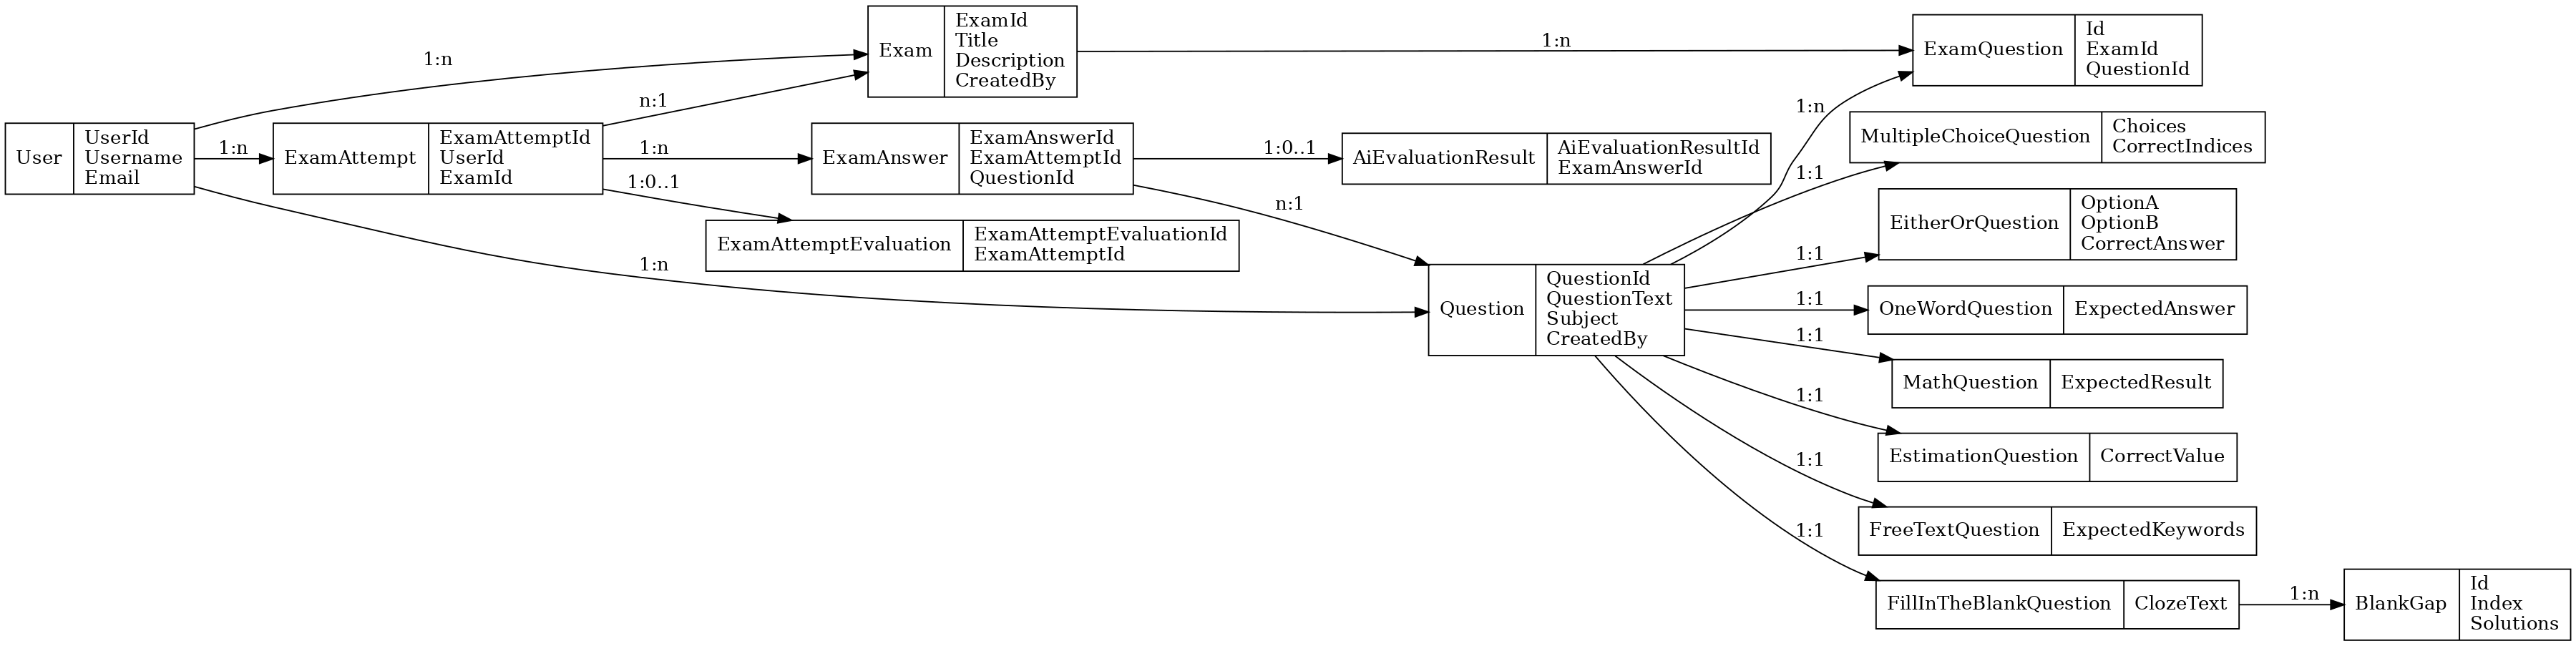
\includegraphics[width=\textwidth]{er_diagram_highres.png}
\caption{Entity-Relationship-Diagramm der GenAI-Bewertungsplattform}
\label{fig:erd}
\end{figure}
\vspace{1em}

Wie in Abbildung~\ref{fig:erd} dargestellt, bilden die Entitäten ein klar strukturiertes und normalisiertes Modell, das eine präzise Trennung zwischen Nutzerinteraktionen, Prüfungsstruktur, Antworten und Bewertungen ermöglicht. Diese Modularität ist entscheidend für die Wartbarkeit des Systems und unterstützt die kontinuierliche Weiterentwicklung. Die Struktur wurde im Verlauf des Projekts schrittweise erweitert, insbesondere im Hinblick auf die Differenzierung von Fragetypen und die Integration des generativen Bewertungssystems. Der aktuelle Stand bietet eine tragfähige Grundlage für zukünftige Erweiterungen wie Fortschrittsanalysen, adaptive Frageauswahl oder erweiterte Feedbackmechanismen.

\subsection{API-Kommunikation}
Die Kommunikation zwischen den verschiedenen Komponenten des Systems folgt dem Prinzip einer serviceorientierten Architektur (SOA) und basiert auf standardisierten RESTful Webservices. Diese Schnittstellen dienen nicht nur der Verbindung zwischen Frontend und Backend, sondern insbesondere auch der Integration externer KI-Dienste, im konkreten Fall der OpenAI-API zur automatisierten Bewertung von Freitext- und anderen offenen Antwortformaten.

\subsubsection{Interne Kommunikation (Frontend–Backend)}
Sobald ein Prüfungsversuch abgeschlossen wurde, werden die im Frontend eingegebenen Antworten als strukturierte Datenobjekte (SubmitExamAttemptDto) an das Backend gesendet. Diese enthalten neben den Antwortinhalten auch Metadaten wie Prüfungs- und Benutzer-IDs. Im Backend erfolgt zunächst die Speicherung der Antworten in der Datenbank. Anschließend werden sie zur Bewertung vorbereitet, indem die relevante Frage mitsamt ihrer Typ-spezifischen Konfiguration (z. B. Multiple-Choice-Optionen oder erwartete Ergebnisse) analysiert und mit den Benutzereinstellungen (Toleranz für Tippfehler, Groß-/Kleinschreibung, Schätztoleranz) angereichert wird.

\subsubsection{Externe Kommunikation (Backend–OpenAI API)}
Die anschließende Auswertung erfolgt durch die Integration der OpenAI-API. Für jede zu bewertende Antwort wird im Backend ein spezifisch strukturierter Prompt generiert, der aus der Frage, der Nutzereingabe, der erwarteten Lösung und den Bewertungseinstellungen besteht. Diese Informationen werden als Teil eines JSON-Objekts an die API gesendet. Der Aufruf erfolgt als HTTP-POST-Anfrage mit einem festgelegten Sprachmodell (z. B. gpt-4), wobei ein rollenbasierter Konversationsverlauf (system und user) verwendet wird, um dem Modell klare Bewertungsanweisungen zu geben.

Die API antwortet mit einer textbasierten Rückgabe, die ein JSON-Fragment enthält, bestehend aus einer numerischen Bewertung (score) im Bereich von 0 bis 1 sowie einem erklärenden Feedback. Das System extrahiert dieses JSON aus der Antwort mithilfe regulärer Ausdrücke und deserialisiert es anschließend in eine interne Bewertungsstruktur (AiEvaluationResult). Diese Ergebnisse werden der entsprechenden Nutzerantwort zugeordnet und persistent gespeichert.

\subsubsection{Sicherheitsaspekte und Architekturmerkmale}
Die API-Schlüssel für den Zugriff auf die OpenAI-API werden über die Konfigurationsdateien des Backends verwaltet und nicht im Quellcode hinterlegt. Die gesamte Kommunikation mit dem externen Dienst erfolgt verschlüsselt über HTTPS. Die REST-API ist durch rollenbasierte Zugriffskontrollen abgesichert, wobei alle prüfungsrelevanten Endpunkte Authentifizierung per JSON Web Token (JWT) voraussetzen.

\subsubsection{Zusammenfassung}
Die API-Kommunikation stellt die zentrale Brücke zwischen Nutzereingabe und KI-gestützter Bewertung dar. Sie erlaubt die dynamische Generierung von Bewertungen durch den OpenAI-Dienst und liefert eine flexible, semantisch fundierte Rückmeldung, die über klassische Antwort-Matching-Algorithmen weit hinausgeht. Die Entkopplung von Benutzeroberfläche, Bewertungskomponente und Speicherlogik ermöglicht eine klare Trennung von Zuständigkeiten, was sowohl die Wartbarkeit als auch die Erweiterbarkeit der Anwendung unterstützt.

\subsection{Teststrategie}

\newpage

\section{Implementierung}
\subsection{Implementierung der Fragetypen}
\subsection{Integration der generativen KI-Bewertung}
\subsection{Datenbankstruktur und Datenmodelle}
\subsection{Entwicklung der Benutzeroberfläche}

\newpage

\section{Evaluierung}
\subsection{Vergleich von GenAI-Lösungen}
\subsection{Leistung und Genauigkeit der Bewertung}
\subsection{Kostenanalyse der verschiedenen KI-APIs}

\newpage

\section{Ergebnisse und Diskussion}
\subsection{Zusammenfassung der Implementierungsergebnisse}
\subsection{Herausforderungen bei der Entwicklung}
\subsection{Potenzial für zukünftige Erweiterungen}

\newpage

\section{Zukünftige Arbeiten und Erweiterungsmöglichkeiten}
\subsection{Adaptive Lernpfade}
\subsection{Integration von Sprach- und Bilderkennung}
\subsection{Mehrsprachigkeit}

\newpage

\section{Fazit}
\subsection{Erfüllung der Projektziele}
\subsection{Bedeutung der Ergebnisse}
\subsection{Ausblick}


\newpage
\nocite{*}
\printbibliography


\end{document}
